\documentclass[a4paper,12pt]{article}
\usepackage[utf8]{inputenc}
\usepackage[T1]{fontenc}
\usepackage[left=3cm, right=1.5cm, top=2cm, bottom=2cm]{geometry}
\usepackage{graphicx}
\usepackage{float}
\usepackage{booktabs}
\usepackage{array}
\usepackage{amsmath, amssymb}
\usepackage{pgfplots}
\pgfplotsset{compat=1.18}
\usepackage[hidelinks]{hyperref}
\usepackage{xurl}
\usepackage{setspace}
\onehalfspacing

% All reported numbers are macros written by tools/report_numbers.py from results/.
% Generated by tools/report_numbers.py from results/. Do not edit.
\newcommand{\MbBLEU}{33.40}
\newcommand{\MbCHR}{53.93}
\newcommand{\MbGM}{42.44}
\newcommand{\MbLO}{39.73}
\newcommand{\MbHI}{44.93}
\newcommand{\MbShort}{49.95}
\newcommand{\MbMedium}{44.55}
\newcommand{\MbLong}{40.20}
\newcommand{\MbDamaged}{41.79}
\newcommand{\MbIntact}{42.72}
\newcommand{\MbPrefix}{48.27}
\newcommand{\MbNum}{0.817}
\newcommand{\MbName}{0.679}
\newcommand{\MbRatio}{0.98}
\newcommand{\MbTooShort}{7}
\newcommand{\MbRep}{5}
\newcommand{\MbEmpty}{0}
\newcommand{\QwBLEU}{25.73}
\newcommand{\QwCHR}{47.56}
\newcommand{\QwGM}{34.98}
\newcommand{\QwLO}{32.33}
\newcommand{\QwHI}{37.55}
\newcommand{\QwShort}{41.62}
\newcommand{\QwMedium}{37.32}
\newcommand{\QwLong}{32.77}
\newcommand{\QwDamaged}{35.49}
\newcommand{\QwIntact}{34.56}
\newcommand{\QwPrefix}{41.14}
\newcommand{\QwNum}{0.777}
\newcommand{\QwName}{0.627}
\newcommand{\QwRatio}{0.93}
\newcommand{\QwTooShort}{6}
\newcommand{\QwRep}{3}
\newcommand{\QwEmpty}{0}
\newcommand{\BtBLEU}{13.64}
\newcommand{\BtCHR}{31.12}
\newcommand{\BtGM}{20.60}
\newcommand{\BtLO}{18.68}
\newcommand{\BtHI}{22.77}
\newcommand{\BtShort}{42.05}
\newcommand{\BtMedium}{22.25}
\newcommand{\BtLong}{16.34}
\newcommand{\BtDamaged}{19.07}
\newcommand{\BtIntact}{21.84}
\newcommand{\BtPrefix}{35.07}
\newcommand{\BtNum}{0.588}
\newcommand{\BtName}{0.526}
\newcommand{\BtRatio}{0.97}
\newcommand{\BtTooShort}{16}
\newcommand{\BtRep}{77}
\newcommand{\BtEmpty}{0}
\newcommand{\BmBLEU}{10.23}
\newcommand{\BmCHR}{26.12}
\newcommand{\BmGM}{16.35}
\newcommand{\BmLO}{14.63}
\newcommand{\BmHI}{18.34}
\newcommand{\BmShort}{33.51}
\newcommand{\BmMedium}{17.96}
\newcommand{\BmLong}{12.95}
\newcommand{\BmDamaged}{14.38}
\newcommand{\BmIntact}{17.95}
\newcommand{\BmPrefix}{28.57}
\newcommand{\BmNum}{0.475}
\newcommand{\BmName}{0.439}
\newcommand{\BmRatio}{0.99}
\newcommand{\BmTooShort}{22}
\newcommand{\BmRep}{84}
\newcommand{\BmEmpty}{0}
\newcommand{\BxBLEU}{10.35}
\newcommand{\BxCHR}{28.55}
\newcommand{\BxGM}{17.19}
\newcommand{\BxLO}{15.44}
\newcommand{\BxHI}{19.15}
\newcommand{\BxShort}{37.59}
\newcommand{\BxMedium}{17.82}
\newcommand{\BxLong}{13.64}
\newcommand{\BxDamaged}{14.86}
\newcommand{\BxIntact}{19.09}
\newcommand{\BxPrefix}{33.09}
\newcommand{\BxNum}{0.561}
\newcommand{\BxName}{0.492}
\newcommand{\BxRatio}{1.19}
\newcommand{\BxTooShort}{4}
\newcommand{\BxRep}{94}
\newcommand{\BxEmpty}{0}
\newcommand{\EnBLEU}{30.26}
\newcommand{\EnCHR}{52.31}
\newcommand{\EnGM}{39.79}
\newcommand{\EnLO}{37.11}
\newcommand{\EnHI}{42.33}
\newcommand{\EnShort}{48.79}
\newcommand{\EnMedium}{40.80}
\newcommand{\EnLong}{37.81}
\newcommand{\EnDamaged}{39.69}
\newcommand{\EnIntact}{39.88}
\newcommand{\EnPrefix}{46.57}
\newcommand{\EnNum}{0.825}
\newcommand{\EnName}{0.672}
\newcommand{\EnRatio}{1.00}
\newcommand{\EnTooShort}{5}
\newcommand{\EnRep}{12}
\newcommand{\EnEmpty}{0}
\newcommand{\DiffQw}{7.35}
\newcommand{\DiffQwLO}{5.52}
\newcommand{\DiffQwHI}{9.07}
\newcommand{\DiffBt}{21.70}
\newcommand{\DiffBtLO}{19.03}
\newcommand{\DiffBtHI}{24.21}
\newcommand{\DiffEn}{2.61}
\newcommand{\DiffEnLO}{0.84}
\newcommand{\DiffEnHI}{4.71}
\newcommand{\MbBestEpoch}{4}
\newcommand{\MbSteps}{88}
\newcommand{\MbGpus}{2}
\newcommand{\MbEffBatch}{16}
\newcommand{\MbTime}{1 h 01 min}
\newcommand{\MbCurve}{(1,26.60) (2,38.21) (3,40.13) (4,43.39) (5,42.62)}
\newcommand{\BtBestEpoch}{20}
\newcommand{\BtSteps}{88}
\newcommand{\BtGpus}{2}
\newcommand{\BtEffBatch}{16}
\newcommand{\BtTime}{6 h 12 min}
\newcommand{\BtCurve}{(1,1.76) (2,5.22) (3,6.76) (4,9.00) (5,9.73) (6,11.48) (7,12.30) (8,13.88) (9,13.35) (10,13.78) (11,16.17) (12,15.56) (13,17.33) (14,18.75) (15,19.94) (16,19.14) (17,19.50) (18,20.17) (19,20.16) (20,20.23)}
\newcommand{\EnsembleSentence}{The three-model ensemble scores 2.61 GM below mBART-50 alone (paired bootstrap, 95\% CI 0.84 to 4.71). This difference is larger than expected from document sampling alone. The documents were taken from: mBART 84, Qwen 48, ByT5 24. Equal votes give two weaker models a majority over the strongest one, so the proposed single model is kept.}
\newcommand{\EnsembleSummary}{An equal-vote MBR ensemble of the three models scored 39.79, against 42.44 for mBART-50 alone. It did not improve on the best single model.}
\newcommand{\WeightsSentence}{The Phase 2 weights are kept by the team but are not part of the archive because of their size (mBART 2.4 GB, ByT5 1.2 GB per model, Qwen adapter 0.16 GB) and are not published. Retraining instructions are in the README.}


\title{Deep Past Challenge --- Translate Akkadian to English\\[4pt]\large Phase 2 report}
\author{Team Yellow Duck Studio}
\date{}

\emergencystretch=3em
\setlength{\belowcaptionskip}{6pt}
\begin{document}
\maketitle
{\singlespacing\tableofcontents}
\newpage

\section{Problem statement}

\subsection{Task description}
The project develops a machine translation system that converts transliterated Old Assyrian cuneiform into English. Old Assyrian is a low-resource, morphologically rich Semitic language. The texts are mostly administrative and commercial records of Assyrian merchants. They contain scribal notation, determinatives and damaged passages.

\subsection{Data source}
The data comes from the Deep Past Initiative competition \cite{deeppast}. All models are trained on the competition file \texttt{train.csv}: 1{,}561 documents with the columns \texttt{oare\_id}, \texttt{transliteration} and \texttt{translation}. The text is used as provided; only rows with an empty source or target would be dropped. Training and validation are at document level, while the competition test set is at sentence level.

\subsection{Evaluation metrics}
The score is the geometric mean (GM) of corpus BLEU \cite{bleu} and corpus chrF++ \cite{chrfpp}:
\begin{equation}
    \mathrm{GM} = \sqrt{\mathrm{BLEU} \times \mathrm{chrF{+}{+}}}.
\end{equation}
Every Phase 2 number in this report is computed by one implementation, \path{common/metrics.py}. It reproduces sacreBLEU \cite{sacrebleu} (BLEU with the 13a tokenizer; chrF++ with character 6-grams, word 2-grams and $\beta=2$), and \path{tests/test_metrics.py} checks this against sacreBLEU 2.6.0.

\subsection{Evaluation protocol}
\label{sec:protocol}
\begin{itemize}
    \item \textbf{One split.} 10\% of the documents: the sorted document ids are shuffled with \path{random.Random(42)} and the first 156 are used for validation, the remaining 1{,}405 for training (\texttt{common/split.py}). Every notebook compares the SHA-256 of the validation ids with a stored value and stops if it differs.
    \item \textbf{One metric}, computed after training on the selected checkpoint against the full, untruncated references.
    \item \textbf{Uncertainty.} 95\% bootstrap intervals over the validation documents and a paired bootstrap against the best system (5{,}000 resamples, seed 12345) \cite{koehn}. Each model was trained once (seed 42), so these intervals do not include training variance.
    \item \textbf{Length limits} follow the 95th percentile of the training documents for each tokenizer (Table~\ref{tab:config}). ByT5 sources are the exception: 93.5\% fit completely, and the others lose at most 33 bytes (the longest source has 1{,}056 bytes and the limit includes the end token); in Phase 1 mBART and ByT5 used 256 for source and target, and Qwen used 512 for the whole sequence.
    \item \textbf{Decoding differs and is part of each system:} mBART and Qwen are decoded greedily, ByT5 with 8 beams.
\end{itemize}

\section{Baselines (existing solutions)}
\label{sec:baselines}

As existing solutions to this translation task we identified three publicly available pretrained models from different families and adapted them: a multilingual subword encoder--decoder, a byte-level encoder--decoder and an instruction-tuned decoder-only LLM. They were chosen because transliterated Akkadian is written in Latin script with many diacritics and is not covered by the pretraining data of general translation models. The three families treat such text differently: subwords of a multilingual vocabulary, raw bytes without a vocabulary, and a large language model with a small trained adapter. All three were trained on the same 1{,}405 documents.

\subsection{mBART-50}
\path{facebook/mbart-large-50-many-to-many-mmt} \cite{mbart}, fully fine-tuned. The language code is \texttt{en\_XX} for source and target because Akkadian has no code. The checkpoint with the highest validation GM (greedy decoding, after each epoch) is kept: epoch \MbBestEpoch.

\subsection{Qwen2.5-7B-Instruct (QLoRA)}
\path{Qwen/Qwen2.5-7B-Instruct} \cite{qwen} with 4-bit NF4 quantization and a LoRA adapter ($r=16$, $\alpha=32$, dropout 0.05) \cite{lora,qlora}. The checkpoint with the lowest validation loss is kept (epoch 2 of 2), because generating all validation documents after each epoch is too slow for a 7B model. The run log shows 44 optimizer steps per epoch and two GPUs, so the effective batch size was 32.

\subsection{ByT5-small}
\path{google/byt5-small} \cite{byt5}, fully fine-tuned on UTF-8 bytes. The checkpoint with the highest validation GM (greedy decoding) is kept: epoch \BtBestEpoch{} of 20.

\begin{table}[H]
    \centering\small
    \caption{Training configuration of the reported runs (seed 42, Kaggle T4). The effective batch is per-device batch $\times$ accumulation $\times$ GPUs.}
    \label{tab:config}
    \begin{tabular}{lccc}
        \toprule
        & \textbf{mBART-50} & \textbf{Qwen2.5-7B} & \textbf{ByT5-small} \\
        \midrule
        Epochs & 5 & 2 & 20 \\
        Learning rate & $5\cdot10^{-5}$ & $2\cdot10^{-4}$ & $2\cdot10^{-4}$ \\
        Batch $\times$ accumulation & $2\times4$ & $1\times16$ & $2\times4$ \\
        GPUs used & \MbGpus & 2 & \BtGpus \\
        Effective batch & \MbEffBatch & 32 & \BtEffBatch \\
        Optimizer steps per epoch & \MbSteps & 44 & \BtSteps \\
        Max source / target & 576 / 448 tokens & 1{,}024 / 448 tokens & 1{,}024 / 1{,}408 bytes \\
        Checkpoint selected by & validation GM & validation loss & validation GM \\
        Decoding & greedy & greedy & 8 beams \\
        Training time & \MbTime & 1 h 53 min & \BtTime \\
        \bottomrule
    \end{tabular}

    \footnotesize For Qwen, 1{,}024 is the limit for prompt, source and target together, and 448 the limit for generated tokens.
\end{table}

\subsection{Comparison of baselines}

\begin{table}[H]
    \centering
    \caption{Baselines on the 156 shared validation documents.}
    \label{tab:baselines}
    \begin{tabular}{lcccc}
        \toprule
        \textbf{Model} & \textbf{BLEU} & \textbf{chrF++} & \textbf{GM} & \textbf{GM 95\% CI} \\
        \midrule
        mBART-50 & \textbf{\MbBLEU} & \textbf{\MbCHR} & \textbf{\MbGM} & \MbLO--\MbHI \\
        Qwen2.5-7B (QLoRA) & \QwBLEU & \QwCHR & \QwGM & \QwLO--\QwHI \\
        ByT5-small & \BtBLEU & \BtCHR & \BtGM & \BtLO--\BtHI \\
        \bottomrule
    \end{tabular}
\end{table}

\begin{figure}[H]
    \centering
    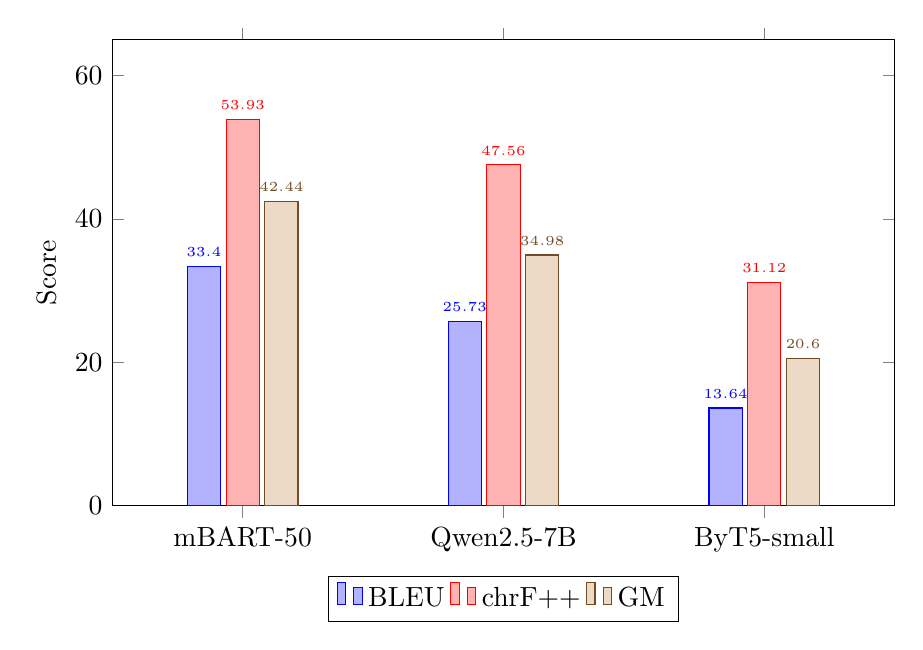
\begin{tikzpicture}
        \begin{axis}[
            ybar, bar width=12pt, width=0.95\textwidth, height=7.5cm,
            ylabel={Score}, symbolic x coords={mbart, qwen, byt5}, xtick=data,
            xticklabels={mBART-50, Qwen2.5-7B, ByT5-small},
            ymin=0, ymax=65, enlarge x limits=0.25,
            legend style={at={(0.5,-0.15)}, anchor=north, legend columns=-1},
            nodes near coords, every node near coord/.append style={font=\tiny},
        ]
        \addplot coordinates {(mbart,\MbBLEU) (qwen,\QwBLEU) (byt5,\BtBLEU)};
        \addplot coordinates {(mbart,\MbCHR) (qwen,\QwCHR) (byt5,\BtCHR)};
        \addplot coordinates {(mbart,\MbGM) (qwen,\QwGM) (byt5,\BtGM)};
        \legend{BLEU, chrF++, GM}
        \end{axis}
    \end{tikzpicture}
    \caption{Validation metrics of the three baselines (same documents, same metric).}
    \label{fig:metrics}
\end{figure}

\paragraph{Analysis.}
mBART-50 is the best baseline on both metrics. Its advantage over Qwen is \DiffQw{} GM (95\% CI \DiffQwLO--\DiffQwHI, paired bootstrap) and its advantage over ByT5 is \DiffBt{} GM (\DiffBtLO--\DiffBtHI). Neither interval includes zero, but both cover only the choice of validation documents, not training variance. The comparison is between complete training recipes with different budgets, not between architectures: ByT5's best checkpoint is its last epoch (Figure~\ref{fig:curves}). Its validation GM flattened only at the end of the 20 epochs, when the linearly decaying learning rate approached zero, so a longer schedule could still improve it.

\section{Proposed model}
\label{sec:proposed}
\textbf{mBART-50} is the proposed model because it has the highest BLEU, chrF++ and GM on the shared validation set (Table~\ref{tab:baselines}).

\subsection{Architecture}
\path{facebook/mbart-large-50-many-to-many-mmt}, a multilingual sequence-to-sequence Transformer, used without architectural changes.

\subsection{Training procedure}
Five epochs, Adafactor, learning rate $5\cdot10^{-5}$, weight decay 0.01, mixed precision (fp16), gradient checkpointing, limits 576/448 tokens. The remaining settings are in Table~\ref{tab:config}, and the exact values are in \path{results/run_mbart50__seed42.json}. Batches are sampled randomly and padded dynamically.

\subsection{Metrics}
BLEU \MbBLEU, chrF++ \MbCHR, GM \MbGM{} (95\% CI \MbLO--\MbHI).

\begin{figure}[H]
    \centering
    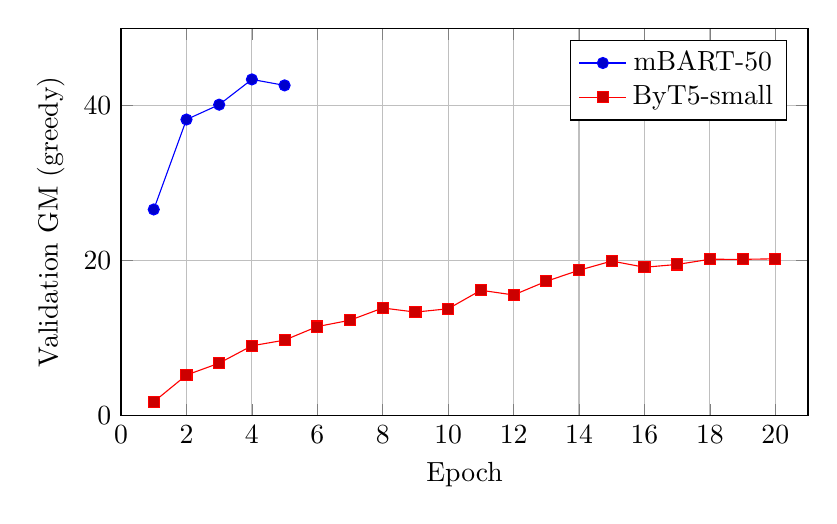
\begin{tikzpicture}
        \begin{axis}[
            width=0.85\textwidth, height=6.5cm, xlabel={Epoch}, ylabel={Validation GM (greedy)},
            xmin=0, xmax=21, ymin=0, ymax=50, legend pos=north east, grid=major,
        ]
        \addplot+[mark=*] coordinates {\MbCurve};
        \addplot+[mark=square*] coordinates {\BtCurve};
        \legend{mBART-50, ByT5-small}
        \end{axis}
    \end{tikzpicture}
    \caption{Validation GM during training, used only to select checkpoints. These values use references truncated to the target limit, so they differ slightly from Table~\ref{tab:baselines}.}
    \label{fig:curves}
\end{figure}

\section{Model improvements}
\label{sec:improvements}
Two changes to the system were tested. Both combine several outputs with Minimum Bayes Risk (MBR) selection \cite{mbr}: the candidate with the highest mean sentence chrF++ against the other candidates is kept. All candidates have an equal vote.

\subsection{Three-model MBR ensemble}
Candidates: the recorded validation predictions of mBART-50, Qwen and ByT5 (one each). The selection uses no references. It was computed with \path{tools/mbr_from_predictions.py} from the recorded predictions, without a joint inference run. The rule is the same as in \path{ensemble-pipeline.ipynb}; that notebook would decode all members with 4 beams and has not been executed in Phase 2. Because all three models are trained on the same split, no validation document is in any member's training data.

\subsection{ByT5 MBR}
A second ByT5 model (\texttt{byt5-member2}, 15 epochs on 1{,}194 of the 1{,}405 training documents) is added to the baseline, and the 5 best beam hypotheses of each model are combined with MBR.

\subsection{Results}
\begin{table}[H]
    \centering
    \caption{Effect of the improvements on the shared validation set.}
    \label{tab:improvements}
    \begin{tabular}{lcccc}
        \toprule
        \textbf{System} & \textbf{BLEU} & \textbf{chrF++} & \textbf{GM} & \textbf{GM 95\% CI} \\
        \midrule
        mBART-50 (proposed model) & \MbBLEU & \MbCHR & \MbGM & \MbLO--\MbHI \\
        MBR ensemble of 3 models & \EnBLEU & \EnCHR & \EnGM & \EnLO--\EnHI \\
        \midrule
        ByT5 baseline & \BtBLEU & \BtCHR & \BtGM & \BtLO--\BtHI \\
        ByT5 member 2 & \BmBLEU & \BmCHR & \BmGM & \BmLO--\BmHI \\
        ByT5 MBR (both models) & \BxBLEU & \BxCHR & \BxGM & \BxLO--\BxHI \\
        \bottomrule
    \end{tabular}
\end{table}

\EnsembleSentence

ByT5 MBR is worse than the ByT5 baseline (\BxGM{} against \BtGM). Its outputs are longer than the references (median length ratio \BxRatio) and contain more repetition loops (\BxRep{} of 156 documents against \BtRep{} for the baseline). A likely cause is that candidates sharing the same repeated text agree with each other, so an agreement-based rule favours them.

\section{Results}
\label{sec:results}

\subsection{Validation results and provenance}
Table~\ref{tab:provenance} links every reported row to the notebook, run record and prediction file. The full registry with hyperparameters and best epochs is \path{results/experiment_registry.md}.

\begin{table}[H]
    \centering\footnotesize
    \caption{Provenance of all reported validation results (seed 42). Files are in \texttt{results/}; predictions are in \texttt{preds\_val\_<system>\_\_seed42.csv}.}
    \label{tab:provenance}
    \begin{tabular}{llll}
        \toprule
        \textbf{Row} & \textbf{GM} & \textbf{Produced by} & \textbf{Run record} \\
        \midrule
        mBART-50 & \MbGM & \texttt{mbart50.ipynb} & \path{run_mbart50__seed42.json} \\
        Qwen2.5-7B & \QwGM & \path{pipeline_QwenQLoRa.ipynb} & \path{run_qwen2.5-7b-lora__seed42.json} \\
        ByT5 baseline & \BtGM & \path{byte-level-seq2seq.ipynb} & \path{run_byt5__seed42.json} \\
        ByT5 member 2 & \BmGM & \path{byte-level-seq2seq.ipynb} & \path{run_byt5-member2__seed42.json} \\
        ByT5 MBR & \BxGM & \path{byte-level-seq2seq.ipynb} & \path{run_byt5-mbr__seed42.json} \\
        MBR ensemble & \EnGM & \path{mbr_from_predictions.py} & \path{run_mbr3-ensemble__seed42.json} \\
        \bottomrule
    \end{tabular}
\end{table}

The Qwen result comes from a run in which the first generation call failed (missing autocast); the predictions were then generated in the same session with autocast. The executed notebook is kept in \path{legacy/executed/}. The submitted notebook contains the fix and completed a short smoke test on Kaggle: it ran to the end without errors with heavily shortened training and generation. The full training was not repeated, so the reported score is that of the recorded run.

\subsection{Error analysis}
Produced by \path{tools/analyze_runs.py} (\path{results/error_analysis.md}). Documents are split into terciles by source length; \emph{damaged} documents contain gap or \texttt{x} markers. Number and name recall are string-based heuristics.

\begin{table}[H]
    \centering\small
    \caption{GM on subsets of the validation documents.}
    \label{tab:subsets}
    \begin{tabular}{lccccc}
        \toprule
        \textbf{Model} & \textbf{Short} & \textbf{Medium} & \textbf{Long} & \textbf{Damaged} & \textbf{Intact} \\
        \midrule
        mBART-50 & \MbShort & \MbMedium & \MbLong & \MbDamaged & \MbIntact \\
        Qwen2.5-7B & \QwShort & \QwMedium & \QwLong & \QwDamaged & \QwIntact \\
        ByT5 baseline & \BtShort & \BtMedium & \BtLong & \BtDamaged & \BtIntact \\
        MBR ensemble & \EnShort & \EnMedium & \EnLong & \EnDamaged & \EnIntact \\
        \bottomrule
    \end{tabular}
\end{table}

\begin{table}[H]
    \centering\small
    \caption{Error statistics. \emph{Length}: median output/reference length in words. \emph{Short}: outputs below half the reference length. \emph{Repetitive}: more than 30\% repeated 4-grams.}
    \label{tab:errors}
    \begin{tabular}{lcccccc}
        \toprule
        \textbf{Model} & \textbf{Numbers} & \textbf{Names} & \textbf{Length} & \textbf{Short} & \textbf{Repetitive} & \textbf{Empty} \\
        \midrule
        mBART-50 & \MbNum & \MbName & \MbRatio & \MbTooShort & \MbRep & \MbEmpty \\
        Qwen2.5-7B & \QwNum & \QwName & \QwRatio & \QwTooShort & \QwRep & \QwEmpty \\
        ByT5 baseline & \BtNum & \BtName & \BtRatio & \BtTooShort & \BtRep & \BtEmpty \\
        ByT5 MBR & \BxNum & \BxName & \BxRatio & \BxTooShort & \BxRep & \BxEmpty \\
        MBR ensemble & \EnNum & \EnName & \EnRatio & \EnTooShort & \EnRep & \EnEmpty \\
        \bottomrule
    \end{tabular}
\end{table}

\begin{itemize}
    \item \textbf{Length.} All models lose quality on longer documents. ByT5 is affected most: GM \BtShort{} on short and \BtLong{} on long documents. On short documents it is close to Qwen.
    \item \textbf{Repetition.} \BtRep{} of 156 ByT5 outputs are repetitive, against \MbRep{} for mBART and \QwRep{} for Qwen. Together with the length effect this is the main weakness of ByT5 here.
    \item \textbf{Facts.} Among the single models, mBART reproduces numbers and names most often, which matters for commercial texts, but it still misses about a third of the names.
    \item \textbf{Damage.} Damaged documents are not consistently harder than intact ones for mBART and Qwen; the differences are small.
\end{itemize}

\subsection{Status of the Phase 1 numbers}
\label{sec:phaseone}
The validation numbers of the Phase 1 report are \textbf{withdrawn}. They came from different validation splits, different metric implementations and, for mBART and ByT5, references truncated to 256 tokens or bytes. They were also not linked to runs. The MLflow records are now exported to \path{results/phase1/mlflow_runs.json}:

\begin{table}[H]
    \centering\footnotesize
    \caption{MLflow runs behind the Phase 1 validation rows and the last Phase 1 run of each model. GM is recomputed from the logged BLEU and chrF. \textbf{The values are not comparable between models or with Phase 2.}}
    \label{tab:phaseone}
    \begin{tabular}{lllccc}
        \toprule
        \textbf{Model} & \textbf{Run} & \textbf{Settings} & \textbf{BLEU} & \textbf{chrF} & \textbf{GM} \\
        \midrule
        \multicolumn{6}{l}{\emph{Source of the Phase 1 tables}} \\
        mBART & \texttt{634d0bbb} & 5 ep., batch 1 & 20.12 & 40.80 & 28.65 \\
        Qwen & \texttt{52ae01a0} & 2 ep., 1$\times$16 & 11.44 & 29.46 & 18.36 \\
        ByT5 & \texttt{2d21940c} & none (logging test) & (12.34) & (45.67) & --- \\
        \multicolumn{6}{l}{\emph{ByT5 runs with the settings described in Phase 1 (10 ep., lr $3\cdot10^{-4}$)}} \\
        ByT5 & \texttt{7ff84a28} & marked failed after evaluation & 25.31 & 43.30 & 33.10 \\
        ByT5 & \texttt{316d7e4e} & finished & 24.42 & 42.75 & 32.31 \\
        \multicolumn{6}{l}{\emph{Last Phase 1 runs (settings of the submitted notebooks)}} \\
        mBART & \texttt{398a01b9} & 5 ep., batch 4 & 22.95 & 48.39 & 33.33 \\
        Qwen & \texttt{4c10e51f} & 2 ep., 1$\times$16 & 8.06 & 25.23 & 14.26 \\
        ByT5 & \texttt{16bd7920} & 20 ep., lr $2\cdot10^{-4}$ & 30.89 & 49.83 & 39.23 \\
        \bottomrule
    \end{tabular}
\end{table}

\paragraph{Correction.}
The ByT5 row of the Phase 1 report (12.34 / 45.67 / 23.74) does not come from a trained model. The matching run \texttt{2d21940c}, named \texttt{mlflow\_debug}, lasted 0.7 seconds, has no parameters, and logged the placeholder values 1.234, 1.567, 12.34 and 45.67. It was a test of the logging connection, and its values were reported by mistake. The rebuttal repeated this run as evidence; that statement was wrong.

\paragraph{Why the ByT5 score is much lower than in Phase 1.}
In Phase 1 ByT5 read and produced at most 256 bytes, and the references were cut to the same length. This truncated 72\% of the sources and 66\% of the translations, so those scores (39.23 above; 33.47 and 36.30 in the review) measure mostly the beginnings of documents, on another split. Phase 2 scores complete documents, which are much longer for a byte-level model. As a rough check, we cut the Phase 2 outputs and references to 256 bytes before scoring: ByT5 then reaches \BtPrefix{} GM instead of \BtGM{} (mBART \MbPrefix, Qwen \QwPrefix). The \BtShort{} GM on short documents points in the same direction. Document length therefore explains part of the drop, but the effect was not isolated in a separate experiment, and the different split, training data and sequence lengths may also have contributed. The two sets of scores must not be compared directly, and they do not show that the ByT5 architecture is unsuitable.

\subsection{Public leaderboard (Phase 1 submissions)}
No new leaderboard submission was made in Phase 2. The Phase 1 submissions scored 28.0895 (mBART-50) and 27.3855 (ensemble). The reviewers obtained 27.9735 and 27.3855 with their reruns. The leaderboard scores sentences, so these values cannot be compared with the document-level validation scores above, and they say nothing about the Phase 2 models.

\section{Reproducibility}
\label{sec:repro}
Step-by-step instructions are in \texttt{README.md}. In short:

\begin{itemize}
    \item \textbf{Without a GPU:} the scores, confidence intervals, ensemble, tables and error analysis are recomputed from \texttt{results/} with the scripts in \texttt{tools/}. \texttt{train.csv} of the competition must be placed in the repository root.
    \item \textbf{Retraining:} \texttt{mbart50.ipynb} (Internet off, third-party base weights attached), \path{byte-level-seq2seq.ipynb} and \path{pipeline_QwenQLoRa.ipynb} (Internet on) run on Kaggle T4~$\times$2. By default they read no secrets and upload nothing.
    \item \textbf{Environment:} package versions and GPUs of each run are in \path{results/env_*.json} (all training runs: Python 3.13.16, PyTorch 2.11.0, transformers 5.20.2, two Tesla T4; Qwen also peft 0.21.2 and bitsandbytes 0.50.2).
    \item \textbf{Weights:} \WeightsSentence{} Scores of retrained models can differ slightly because GPU training is not fully deterministic.
    \item \textbf{Consistency checks:} \path{tools/sync_shared_cells.py} \texttt{-{}-check} verifies that all notebooks contain the same split, metric and logging code; \texttt{pytest tests/} checks the metric against sacreBLEU and the MBR rule.
\end{itemize}

The \texttt{preprocessing/} directory builds a sentence-level dataset that was not used for any reported model.

\section{Conclusion}

\subsection{Summary of findings}
\begin{itemize}
    \item On one shared validation set and one metric, \textbf{mBART-50} is the best of the three baselines (GM \MbGM), followed by Qwen2.5-7B with QLoRA (\QwGM) and ByT5-small (\BtGM). The order of the last two is the reverse of the one given in the Phase 1 report.
    \item \EnsembleSummary
    \item MBR over two ByT5 models reduced the score (\BxGM{} against \BtGM), probably because repeated text reinforces itself in an agreement-based selection.
    \item The main problems are long documents, proper names and, for ByT5, repetition loops.
\end{itemize}

\subsection{Limitations}
\begin{itemize}
    \item \textbf{One seed per model.} Training variance was not measured.
    \item \textbf{One validation split}, which was also used to select checkpoints. The scores are therefore slightly optimistic.
    \item \textbf{Different training budgets and decoding.} The result ranks training recipes, not architectures. ByT5 reached its best score in the last epoch, and Qwen was trained for only 2 epochs.
    \item \textbf{Ensemble from recorded outputs} with each member's own decoding; not run on the test set.
    \item \textbf{No new leaderboard submission}, and the Phase 2 weights are not published. The mBART test-time inference uses 5 beams, unlike the greedy validation decoding, and was not evaluated; one of its four sample-test outputs is a repetition loop.
    \item \textbf{Document-level training}, while the competition scores sentences.
    \item \textbf{Automatic metrics only.} No Assyriologist checked the translations, and there was no systematic hyperparameter search.
\end{itemize}

\subsection{Future work}
Repeat the training with several seeds; train ByT5 longer and constrain repetition during decoding; train on the sentence-level data; compare decoding settings for all models; combine n-best lists of mBART and Qwen; test task-adaptive pretraining and back-translation.

\begin{thebibliography}{99}\small
\bibitem{deeppast} Deep Past Initiative Machine Translation, Kaggle competition. \url{https://www.kaggle.com/competitions/deep-past-initiative-machine-translation}
\bibitem{mbart} Y. Tang et al. Multilingual Translation with Extensible Multilingual Pretraining and Finetuning. arXiv:2008.00401, 2020.
\bibitem{byt5} L. Xue et al. ByT5: Towards a Token-Free Future with Pre-trained Byte-to-Byte Models. TACL, 2022.
\bibitem{qwen} Qwen Team. Qwen2.5 Technical Report. arXiv:2412.15115, 2024.
\bibitem{lora} E. J. Hu et al. LoRA: Low-Rank Adaptation of Large Language Models. ICLR, 2022.
\bibitem{qlora} T. Dettmers et al. QLoRA: Efficient Finetuning of Quantized LLMs. NeurIPS, 2023.
\bibitem{bleu} K. Papineni et al. BLEU: a Method for Automatic Evaluation of Machine Translation. ACL, 2002.
\bibitem{chrfpp} M. Popovi\'c. chrF++: words helping character n-grams. WMT, 2017.
\bibitem{sacrebleu} M. Post. A Call for Clarity in Reporting BLEU Scores. WMT, 2018.
\bibitem{mbr} S. Kumar and W. Byrne. Minimum Bayes-Risk Decoding for Statistical Machine Translation. HLT-NAACL, 2004.
\bibitem{koehn} P. Koehn. Statistical Significance Tests for Machine Translation Evaluation. EMNLP, 2004.
\end{thebibliography}

\end{document}
